\documentclass[12pt, hyperref={unicode}]{beamer}
 
\usepackage[czech]{babel}
\usepackage[utf8]{inputenc}
\usepackage{graphicx}
\usepackage{algorithm}
\usepackage{algorithmic}
\usepackage{hyperref}
\usepackage{xcolor}
\usetheme{Pittsburgh}



\graphicspath{{images/}} 

\title{Grafové algoritmy \\ Jarníkův (Primův) algoritmus}
\author{Matej Mištík (xmisti00)}
\institute{Vysoké učení technické v Brně \\  Fakulta informačních technologii}
\date{\today}

\begin{document}

\begin{frame}
	\titlepage
\end{frame}

\begin{frame}
	\frametitle{Historie}
	\begin{itemize}
		\item  Poprvé algoritmus popsal \textcolor{red}{Vojtěch Jarník roku 1930}, později byl znovuobjeven roku \textcolor{red}{1957 Robertem Primem} a~poté ještě jednou roku \textcolor{red}{1959 Edsgerem Dijkstrou}. V~zahraničí se téměř výlučně používá označení Primův algoritmus, vzácně pak Jarníkův algoritmus nebo DJP algoritmus.
	\end{itemize}	
\end{frame}

\begin{frame}
	\frametitle{Jak funguje ?}
	\begin{itemize}
		\item Problém minimální kostry. 	
		\pause		
		\item Nehledáme nejkratší spojení mezi dvěma vrcholy
	    ~jako~při~Dijkstrovým algoritmu.
		\pause
		\item Hledáme totiž nejkratší cestu mezi všemi vrcholmi najednou.
		\item Je to takzvaná \textbf{MST} \uv{minimum spanning tree} nebo ~v~ překladů \textcolor{red}{minimální kostra}.
	\end{itemize}
		
\end{frame}



\begin{frame}
	\frametitle{Janíkův Algoritmus}
	\begin{enumerate}	
		\item Zvolíme $(x, e) \in U$ takové, že $w(e)$ je minimální          (kde~$w(\emptyset)=0$ ). \\
		 Odebereme $U \leftarrow U \backslash\{(x, e)\}$.
			\pause
		\item Přidáme $E(T) \leftarrow E(T) \cup\{e\}$ (nová hrana do budoucí kostry).
			\pause
		\item Pro všechny hrany $f \in E(G)$ vycházející z $x$ provedeme:\\
		    -~Nechť $y$ je druhý konec hrany $f=x y$
		    \\
		    -~Pokud $\left(y, f^{\prime}\right) \notin U,$ nebo $\left(y, f^{\prime}\right) \in U$ pro nějaké $w\left(f^{\prime}\right)>w(f)$
	\end{enumerate}	
		
\end{frame}

\begin{frame}
	\frametitle{Pseudokód}
	
	\begin{algorithmic}[1]
	 \STATE $S \leftarrow\{v\}, T \leftarrow \emptyset$
		\WHILE {$S  \neq V$}
			\STATE vrcholy $i \in V \backslash S$ a $j \in S$, pro které je váha hrany $e = {i, j}$
			\STATE nejmenší mezi všemi hranami $\{k, l\},$ kde $k \in V \backslash S$ a $l \in S$
		\ENDWHILE
	\end{algorithmic}
\end{frame}


\begin{frame}
	\frametitle{Ukázka}
	\centering
	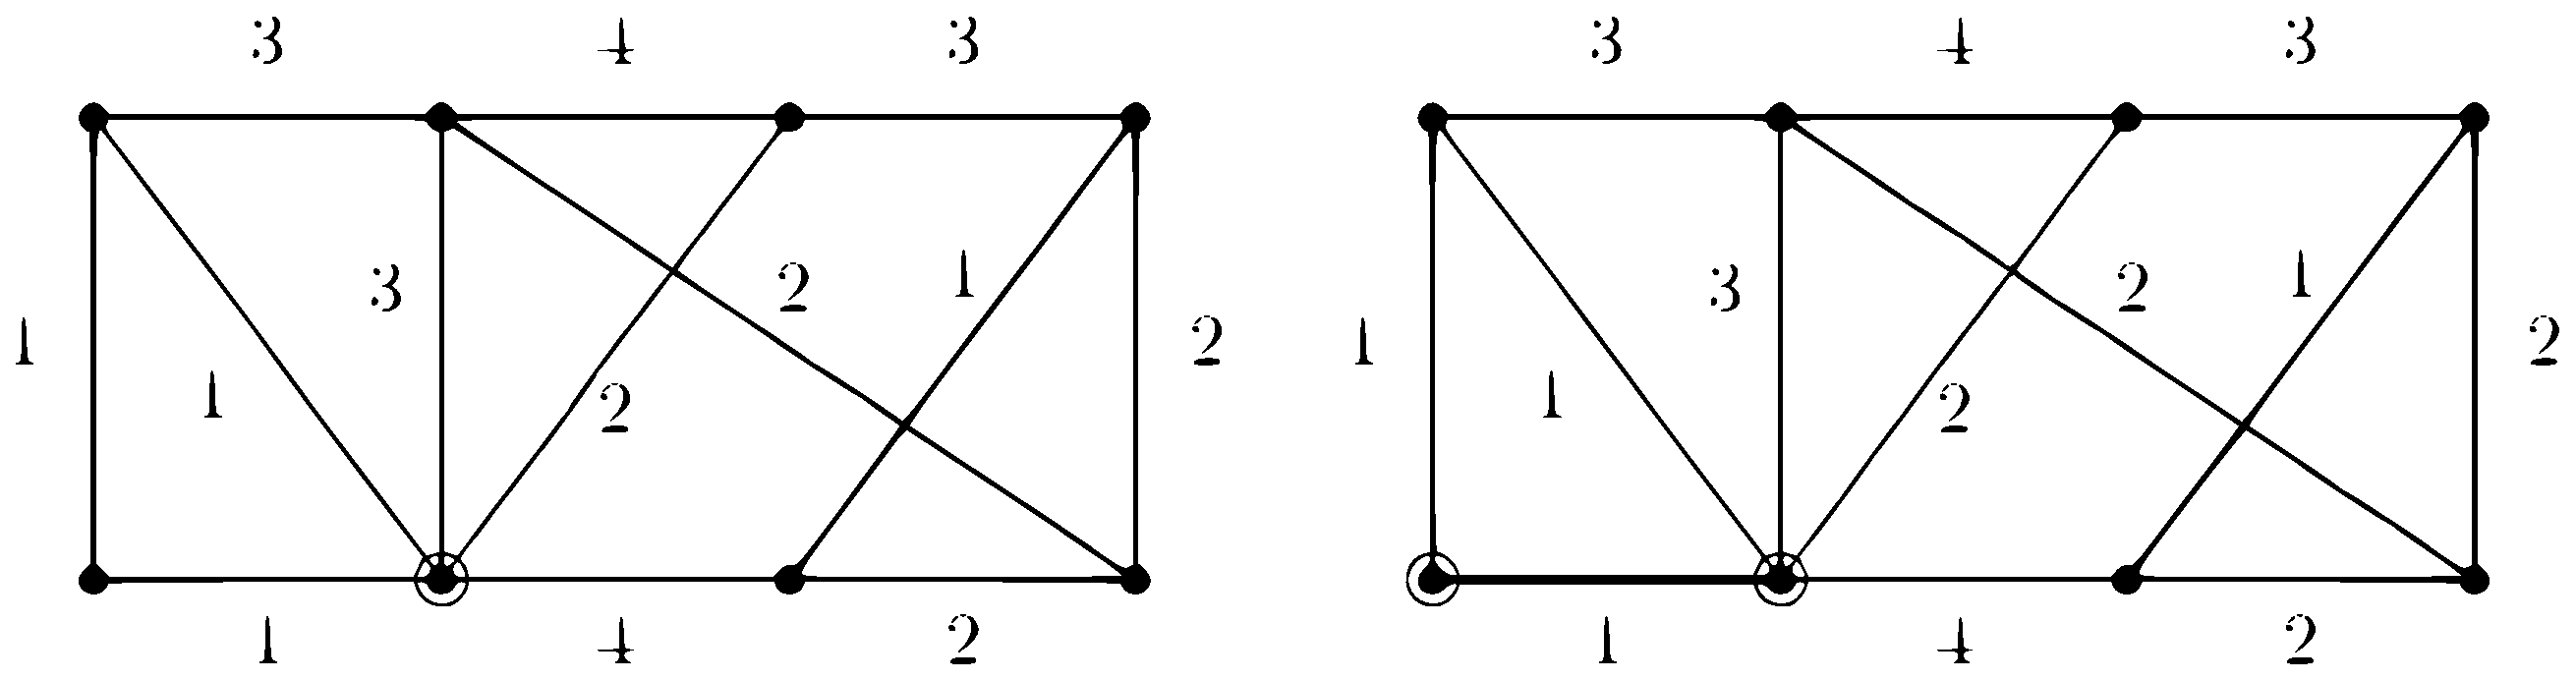
\includegraphics[scale=0.33]{first.eps}
	\pause
	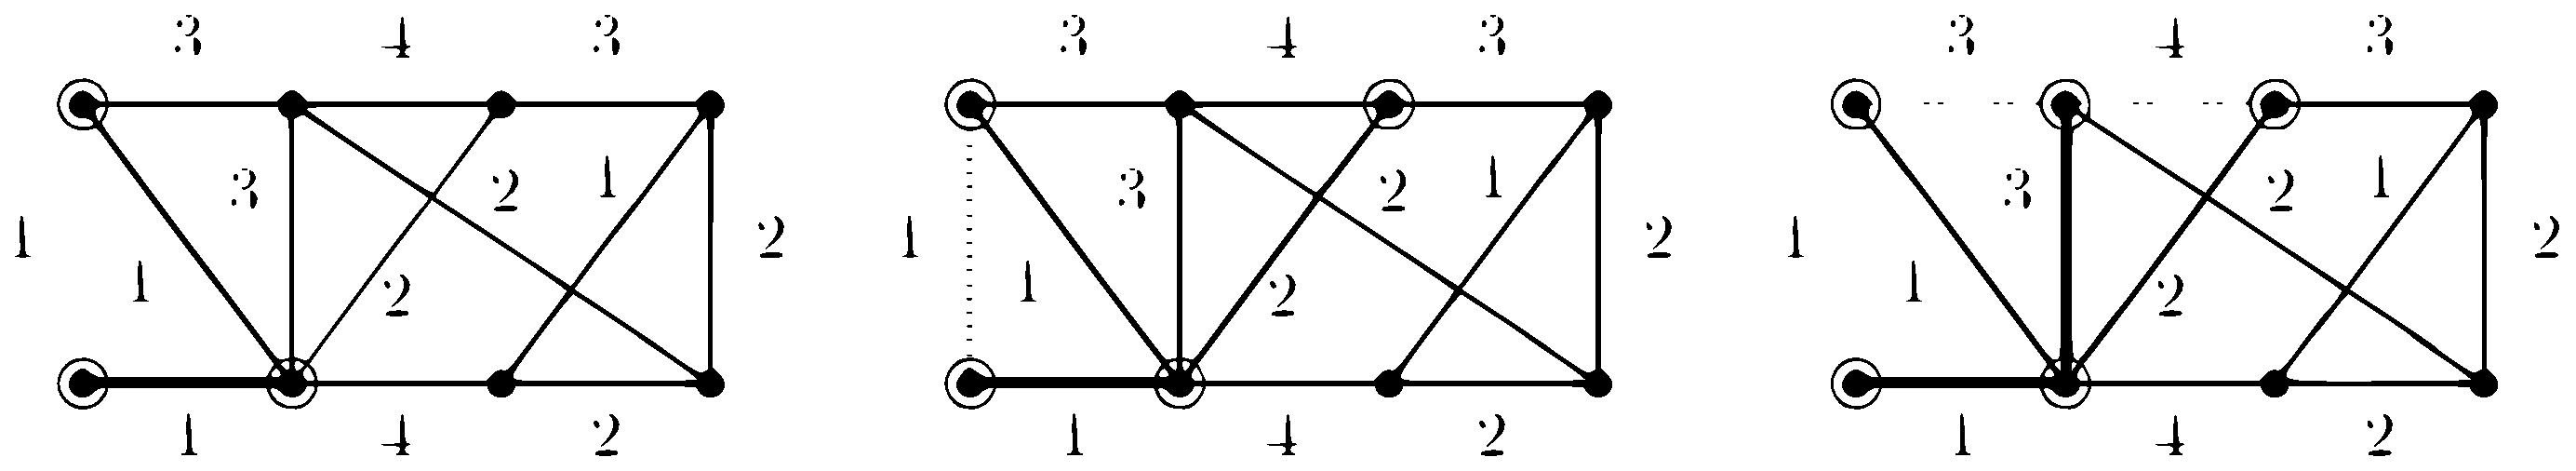
\includegraphics[scale=0.33]{second.eps}
	\pause
	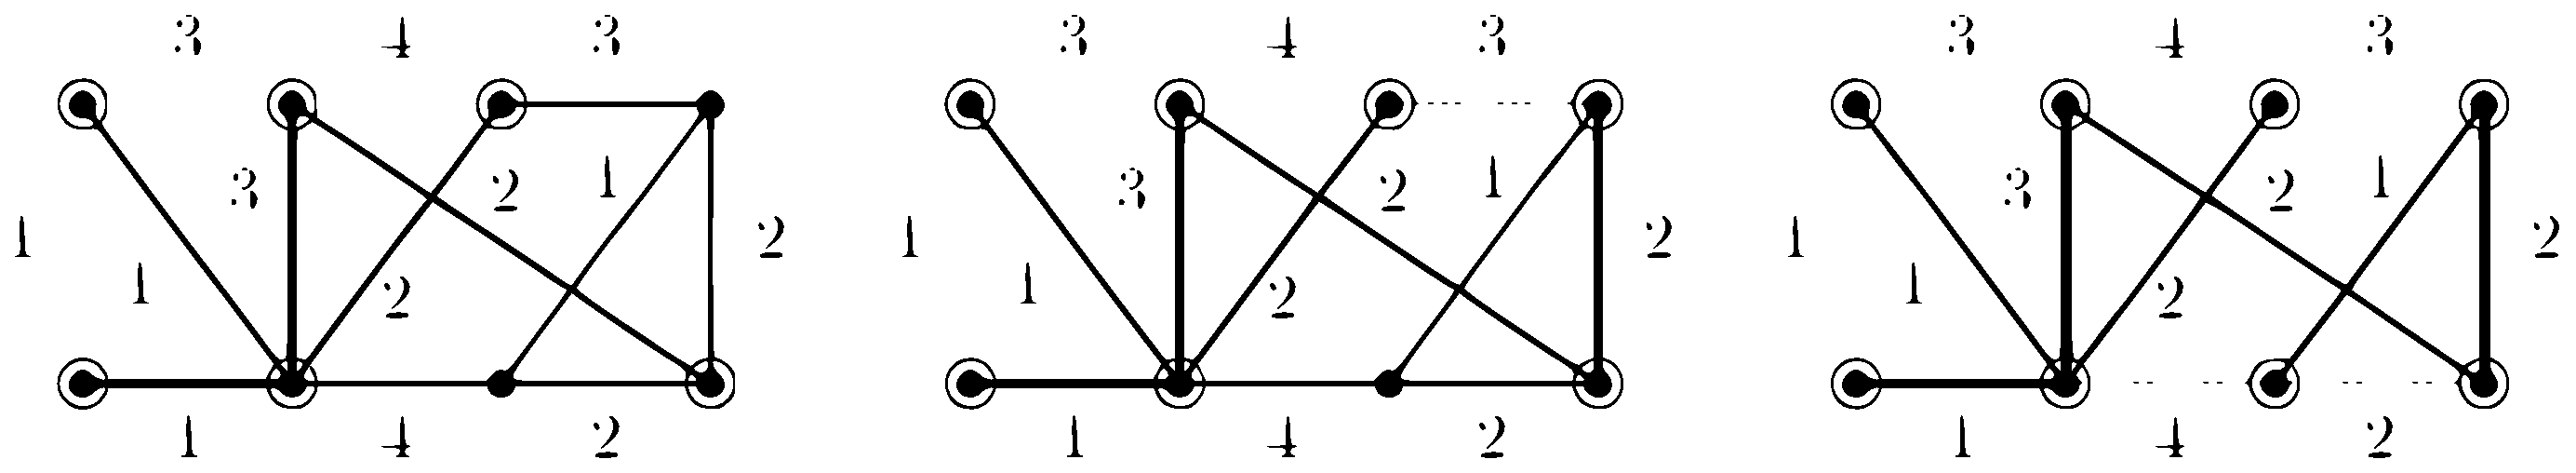
\includegraphics[scale=0.33]{third.eps}		
\end{frame}

\begin{frame}
	\frametitle{Zdroje}
	\begin{itemize}
		\item Referenční zdroje \\
			\url{https://prase.cz/library/GrafoveAlgoritmyPK/GrafoveAlgoritmyPK.pdf} 
	\end{itemize}
\end{frame}
\end{document}